 %%%%%%%%%%%%%%Empieza la presentacion%%%%%%%%%%%%%%%%%%%%%%%%%%%%%%%%%%%%

%\begin{frame}
%\frametitle{Esquema}
 %   \tableofcontents
%\end{frame}

\section{Introducción}


\begin{frame}\frametitle{Señales deterministas y estocásticas I}
    \footnotesize
    \begin{itemize}
        \item \alert{Señales deterministas}: 
        \begin{itemize}\footnotesize
            \item Toman siempre el mismo valor para el mismo instante de tiempo. 
            \item Se representan por una única secuencia continua/discreta de valores. 
            \item El valor en cada instante puede ser definido de forma explícita.
            \item Función matemática determinista:  $t \rightarrow f(t)$\\\scriptsize\color{gray} \emph{relaciona el valor de la señal con el valor de variable independiente (tiempo).}
        \end{itemize}
        \item \alert{Señales estocásticas/aleatorias}: 
        \begin{itemize}\footnotesize
            \item No toman siempre el mismo valor para un mismo instante de tiempo. 
            \item Colección infinita de secuencias continuas/discretas de valores. 
            \item El valor en cada instante es una variable aleatoria.
            \item El comportamiento se define a través de una función de probabilidad.
        \end{itemize}
    \end{itemize}
\end{frame}

%%%%%%%%%%%%%%%%%%%%%%%%%%%%%%%%%%%%%%%%%%%%%%%%

\begin{frame}\frametitle{Señales deterministas y estocásticas II}
    \begin{columns}[T]
        \begin{column}{6cm}
            \small
            \centering Señal determinista:\\
            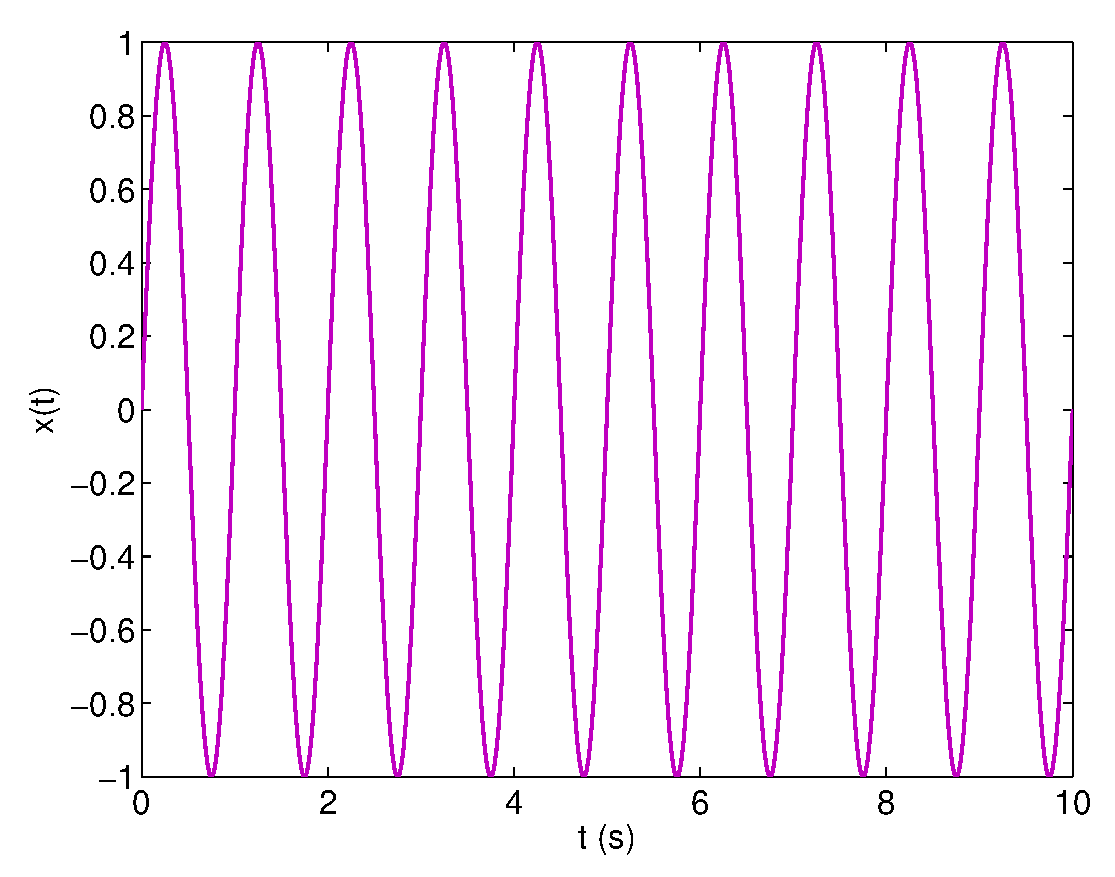
\includegraphics[width=6cm]{./Figures/SignalDeterministic.eps} 
            $x(t)=sen(\omega t)$
        \end{column}
        \begin{column}{6cm}
            \small
            \centering Señal estocástica:\\
            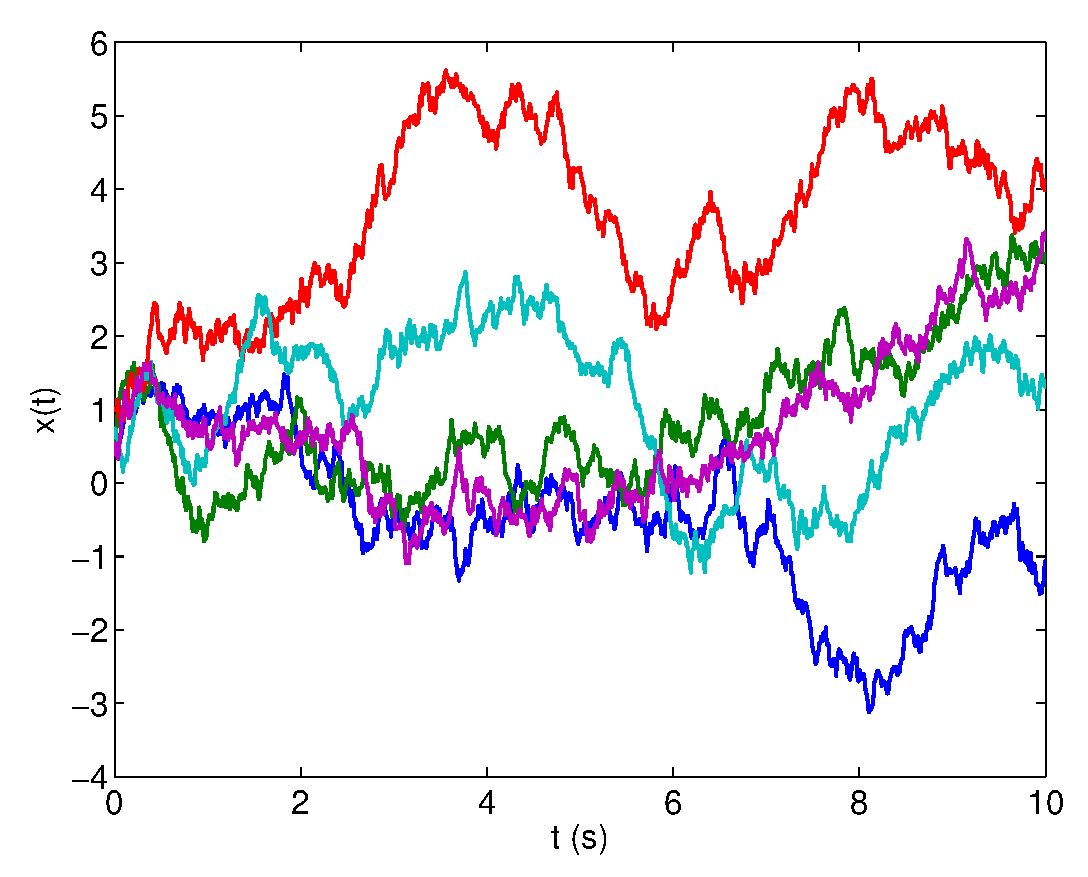
\includegraphics[width=6cm]{./Figures/SignalRandom.eps}\\
            $p(x(t_0),x(t_1),x(t_2),\dots,x(t_\infty))$
        \end{column}
    \end{columns}
\end{frame}

%%%%%%%%%%%%%%%%%%%%%%%%%%%%%%%%%%%%%%%%%%%%%%%


\begin{frame}\frametitle{Señales deterministas y estocásticas III}
    \begin{itemize}
        \item ¿Las señales reales son deterministas o estocásticas?
        \vspace{0.1cm}
        \begin{itemize}\footnotesize
            \item \alert{Argumento 1:} No existen señales totalmente deterministas.
            \begin{itemize}\scriptsize
                \item Puede existir algún fenómeno que no haya sido tenido en cuenta.
                \item Los valores de la señal no están totalmente determinados a priori.
            \end{itemize}
            \item \alert{Argumento 2:} Todas las señales son intrínsecamente deterministas.
            \begin{itemize}\scriptsize
                \item Desconocimiento parcial del proceso que las genera. 
                \item Por tanto no son realmente aleatorias.
            \end{itemize}
        \end{itemize}
        \vspace{0.1cm}
        \item Clasificación \alert{determinista} vs. \alert{estocástica}:
        \vspace{0.1cm}
        \begin{itemize}\footnotesize
            \item Atiende al tratamiento que se le desea dar a la señal,
            \vspace{0.1cm}
            \item No a la forma en que la señal ha sido generada.
        \end{itemize}
    \end{itemize}
\end{frame}